\subsection{Aclaraciones}
En todos lo experimentos, para cada tamaño de secuencia se corrió el programa 50 veces, guardando el tiempo de cada ejecución. Para elegir un valor representativo de la muestra tomo la \textbf{media} de cada tamaño. (También llamado \textit{promedio}).

La generación de secuencias aleatorias de tamaño $n$ fue hecho en Python3 usando: 
\begin{center}
\begin{tabular}{c}
\begin{lstlisting}[language=Python]
[random.randrange(cota_superior) for _ in range(n)]
\end{lstlisting}
\end{tabular}
\end{center}

donde $cota\_superior$ es un número lo suficientemente grande para que no condicione la muestra. En el gráfico, el valor usado como cota es 1000000.

\subsection{Aleatorias}

Podemos observar una clara diferencia entre los algoritmos de backtracking y los algoritmos de programación dinámica. Esto es lo esperado si tenemos en cuenta que en nuestro análisis original concluímos que los primeros tenían complejidad \textbf{exponencial}, mientras que los segundos tenían complejidad \textbf{polinomial}. \\

{\centering
  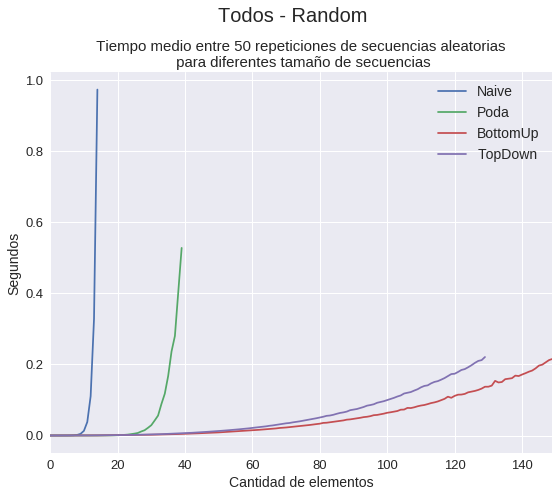
\includegraphics[width=0.75\textwidth]{informe/img/experimentos/todos-random.png} \\
} 

Era esperable que el algoritmo con \textit{poda} sea mucho mas eficiente que el algoritmo \textit{naive}, pero veamos mas de cerca que pasa con los de programación dinámica: \\

{\centering
  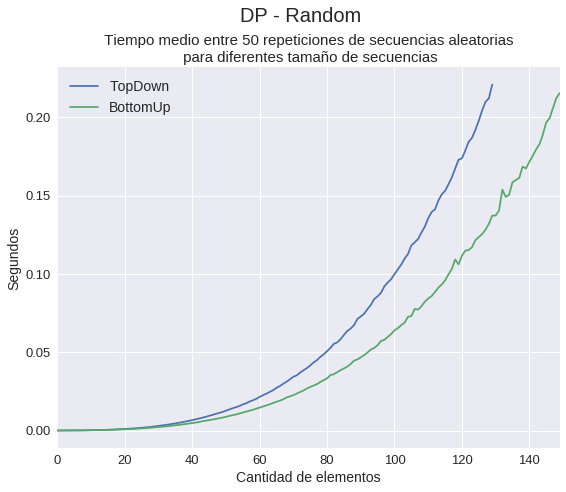
\includegraphics[width=0.75\textwidth]{informe/img/experimentos/dp-random.png} \\
}

Para instancias de tamaño $\leq 40$ \textit{BottomUp} y \textit{TopDown} se comportan de manera muy similar, pero para tamaños mas grandes las curvas comienzan a separarse. \\

En el análisis teórico, tanto \textit{TopDown} como \textit{BottomUp} tenían la misma complejidad. Lo que podemos deducir de estas mediciones es que \textit{TopDown} tiene una constante oculta mas elevada. Esto es razonable ya que en esta técnica se realizan llamados recursivos y en \textit{BottomUp} no. \\

Veamos que pasa con algunos casos particulares de instancias